\documentclass[11pt]{article}

\usepackage{graphicx, epsfig}
\usepackage{amsmath, amssymb, latexsym}
\usepackage[english]{babel}
\usepackage{amssymb}   
%\usepackage{graphicx}
%\usepackage{float} 






% Make a larger page (shrink the margins)
%
\setlength{\textwidth}{6.7in}
\setlength{\textheight}{9.0in}
\setlength{\evensidemargin}{0.0in}
\setlength{\oddsidemargin}{0.0in}
\topmargin -0.5in
\footskip 0.5in



\title{Final Report}
\author{Eric Davis}
\begin{document}
\maketitle
\medskip



\section{Time Profiles}
\hspace{0.5cm}

Over the past several months I have compared the imaging properties of the all MSP`s at the various sites. To do this, I chose to image Jupiter as it was radiant enough to be apparent above the background noise, and could be tracked over several months. By creating a code to produce keograms for the various filters I could compare the sites optics. Specifically, I created space averaged time profiles as Jupiter passed through photometers field of view, which corresponds to approximately 4 degrees. Generally for the time profiles I averaged over five to six bins (or columns) of the keograms, and used the Gaussfit function to come up with the time (row) of Jupiter`s crossing. The time and space profiles were extremely Gaussian in shape, and for almost all samples they fit the curves tremendously well.  As well, the Gaussfit function supplies five values detailing the properties of the curve. The properties of the values are given by:

\begin{eqnarray}
z=\frac{x-A_1}{A_2}  \\
f(x)=A_0e^\frac{-z^2}{2}+A_3+A_4x+A_5x^2
\end{eqnarray}

So $A_0$ provides the amplitude of the Gaussian above the background noise. As well, the full-width-half-maximum can be calculated by $2\sqrt{2\ln(2})A_2$ .  Each site has a spreadsheet labeled "*site name* time profiles." This has all the Gaussian parameters for every filter, as well as what values were used in the IDL code to get said numbers. These time profiles provided an exact transit row, which for the most part translates directly into a transit time as each row in a one hour keogram corresponded to about 30 seconds. However, there is some data that does not start exactly when the file name says they should. Any time I needed an exact transit time I checked the time when the data collection started to guarantee the correct result. 

\begin{figure}[t]
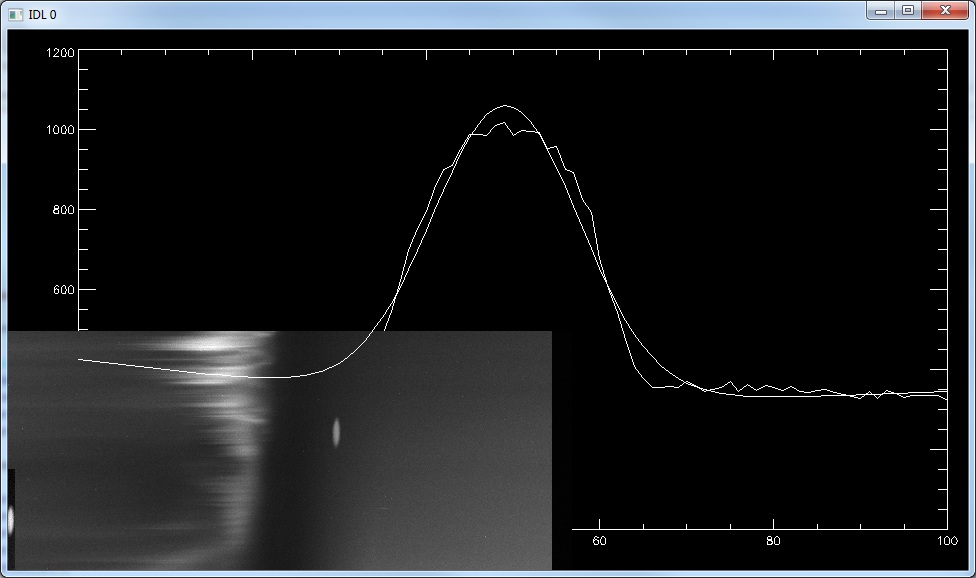
\includegraphics[scale=0.65]{fortsmith_1106_timeprofile.jpg}
\caption{The keogram shows two hours worth of data for an average night at the Fort Smith site. Time runs vertically in the image. Subset within the keogram is the actual slice of the data that includes Jupiter and was used for producing the plot. The subset image in this particular figure is averaged over six bins and then the resulting numbers are plotted as a function of time (row number). Also displayed is a plot of the equation produced using the Gaussfit function. Even in this example it is easy to see the time profiles of Jupiter are quite Gaussian.}
\end{figure}


There was only a couple hitches with the Gillam data. All the data in late 2011 I used in the time profiles had chunks of data missing. Unfortunately, the missing chunks corresponded to either steps missing in the "mirrror\_step" or "time" part of the array. So a lot of time was spent making a code that checked both and then selected which part correctly predicted amount of missing data.  


\begin{figure}[h!]
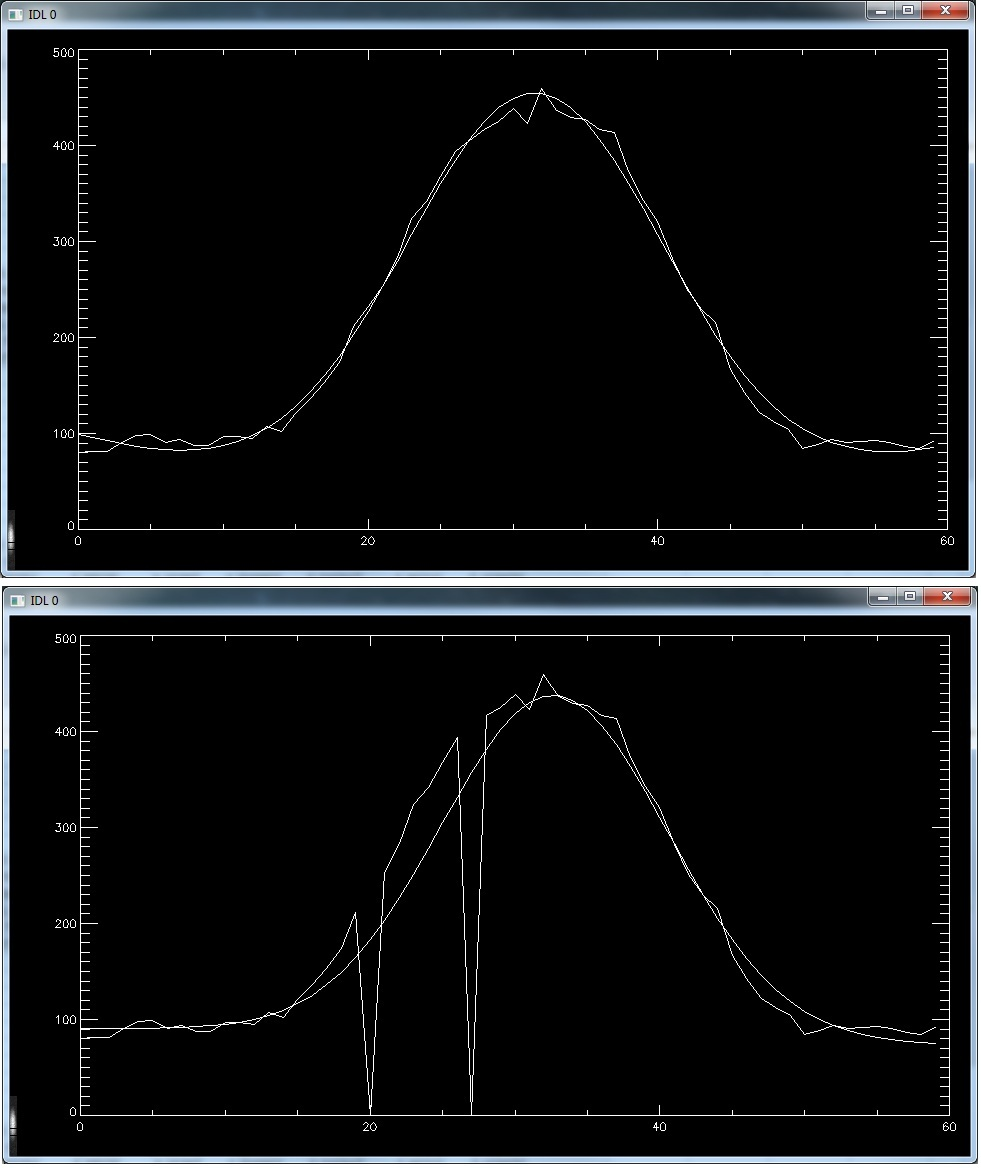
\includegraphics[scale=0.6]{gillam_with_avg_fill_vs_original_fill.jpg}
\caption{Just a comparison from where the missing data was filled in with zeroes, which skewers the Gaussfit function just enough to warrant fixing it. In the top image the missing data is averaged from the rows above and below, which is easily seen to provide a more accurate Gaussian fit. }
\end{figure}



The transit times also could be used for figuring out the alignment of the photometers. By using SkyCalc you can plug in specific times, as well as coordinates of any astronomical body, and it will show you where that object would be if you were looking at the sky at that particular place and time. Ideally, the instruments would follow the geographic north and south poles. However, out in the field tends to be less than ideal, and the instruments are all pointed in slightly different directions. SkyCalc allowed me to look at the azimuth, which at the geographic north pole is 0$^\circ$, the south is 180$^\circ$ and centered around a point somewhere between the south horizon and the north star. Plugging in transit times for Jupiter in SkyCalc and subtracting 180$^\circ$ from the resulting azimuth of Jupiter gives an accurate measurement for the angular separation of the instruments alignment to the geographic North-South meridian.


\section{Space Profiles}

Using a similar process as before, I took Gaussian profiles of Jupiter as a function of bin number. These are much steeper Gaussian curves. These space profiles provided the angle above the horizon Jupiter appeared to be at the four sites. This can then be compared to the angle given by SkyCalc for Jupiter at the transit times recorded by the microspectrophotometer. 



\begin{figure}[h!]
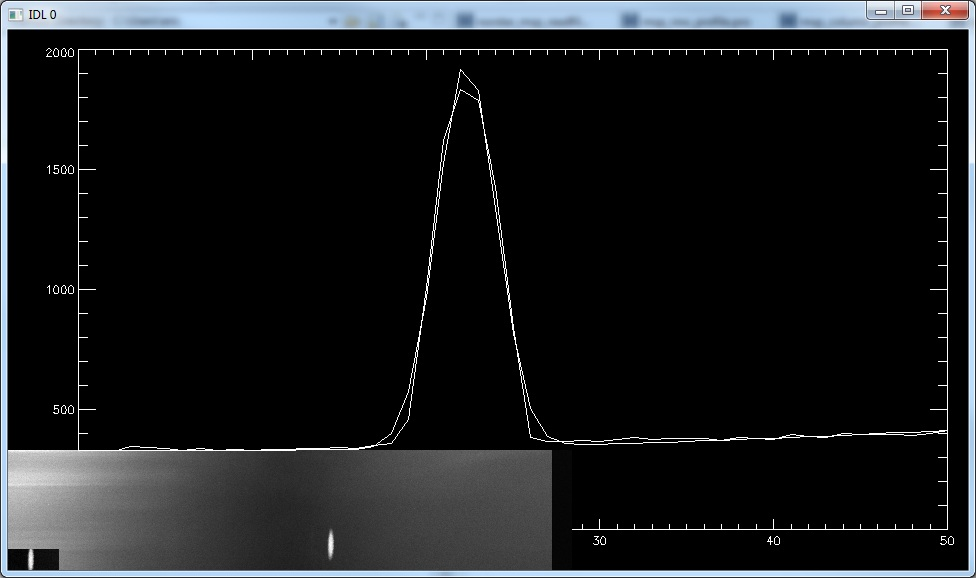
\includegraphics[scale=0.65]{spaceprofile_athabasca_1215.jpg}
\caption{This is space profile of Jupiter from the Athabasca site on 12/15/2011. Similar to before, although this time we are looking at a single hour. The inset image within the keogram is what was plotted in the background. This time all the rows are averaged and the data is plotted as a function of space (bin number). Again, the expression given by the Gaussfit function is overlaid with the actual plot of data.}
\end{figure}

\section{Imaging Results}

\begin{figure}[h!]
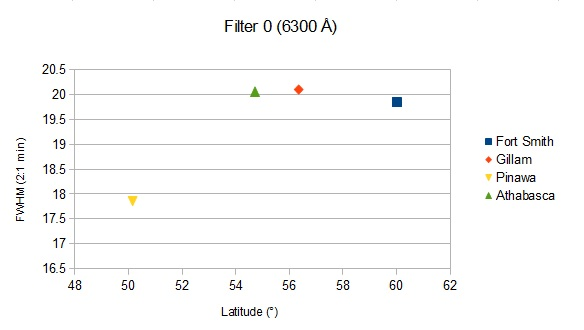
\includegraphics[scale=1.0]{filter0_FWHM.jpg}
\end{figure}

\begin{figure}[h!]
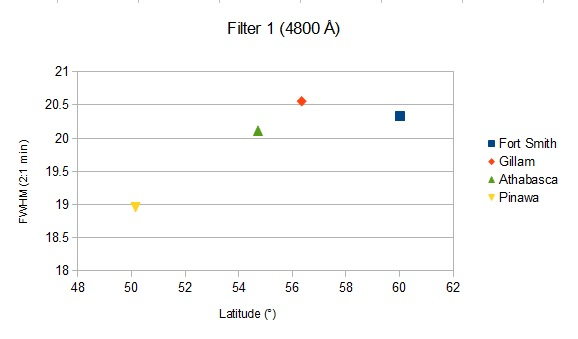
\includegraphics[scale=1.0]{filter1_FWHM.jpg}
\end{figure}

\begin{figure}[h!]
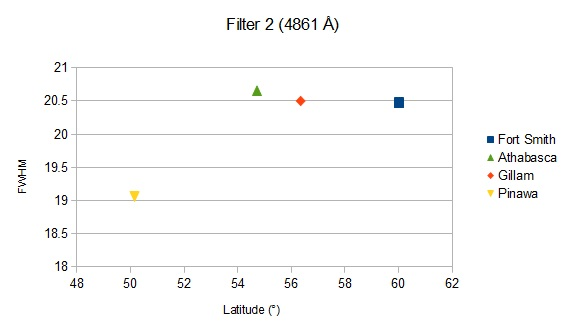
\includegraphics[scale=1.0]{filter2_FWHM.jpg}
\end{figure}

\begin{figure}[h!]
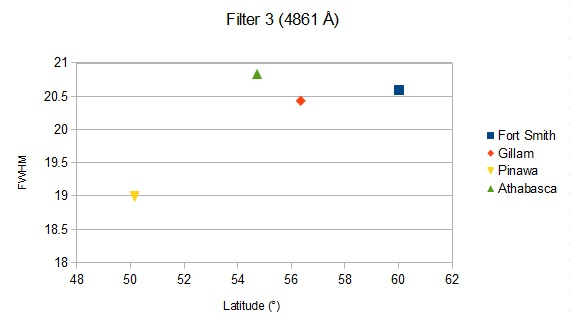
\includegraphics[scale=1.0]{filter3_FWHM.jpg}
\end{figure}

\begin{figure}[h!]
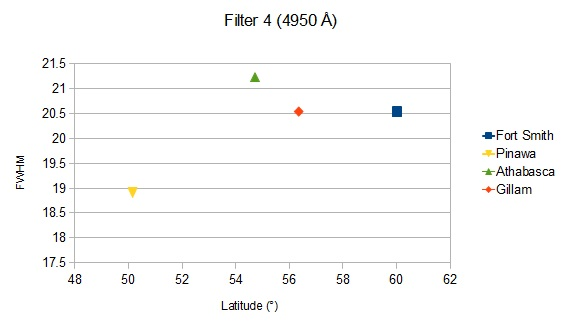
\includegraphics[scale=1.0]{filter4_FWHM.jpg}
\end{figure}

\begin{figure}[h!]
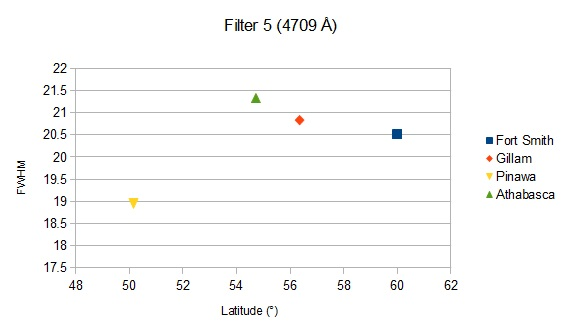
\includegraphics[scale=1.0]{filter5_FWHM.jpg}
\end{figure}

\begin{figure}[h!]
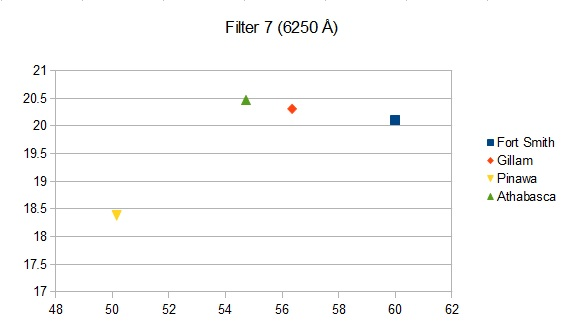
\includegraphics[scale=1.0]{filter7_FWHM.jpg}
\end{figure}


\hspace{0.5cm}
Using only the parameter $A_2$ from the Gaussfit, I calculated the FWHM for each filter on a variety of dates for every site.  Ideally each site should approximately have the same FWHM's for Jupiter as a function of time. This comparison was a check, and the results are below as plots. The plots are averages of FWHM's from several nights, with the outliers removed for atmospheric or other random effects. All plots  have at least five nights of data being averaged. For the plots that are missing labels, the X-axis is always latitude in degrees. The Y-axis is the row (time), where 2 rows equals one minute.

\hspace{0.5cm}

For the most part, the results were consistent between Fort Smith, Gillam, and Athabasca. On the other hand, Pinawa consistently had a FWHM that was a 30 seconds to a minute smaller than the other sites. This would indicate that the imaging system, likely the optics, of the instruments at Pinawa have been set up differently. All four sites have a spreadsheet containing all the data that was used and analyzed to produce the plots. All spreadsheets have "time profile" in the name. These profiles also contain the transit row (transit time) for all the profiles. However, not every set of data begins at the time listed in the file name. For example, it might be labeled as UT 3 but the actual data starts at UT 3:21. Actual transit times (verified by checking exactly what time the data file starts) are contained as a decimal in the "space profile" spreadsheets. These exact times were necessary to analyze the predicted position of Jupiter in the sky verses what the instruments measured, as discussed below.



\begin{figure}[h!]
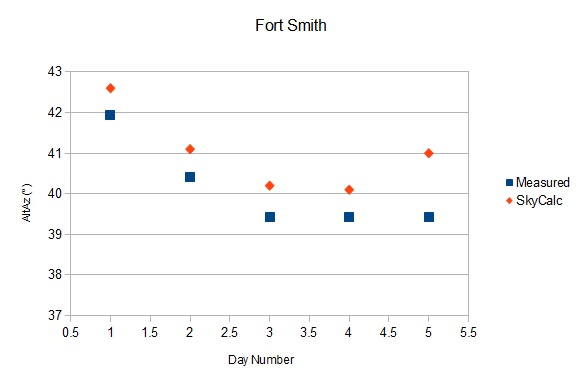
\includegraphics[scale=1.0]{fortsmith_AltAz_comparison.jpg}
\end{figure}

\begin{figure}[h!]
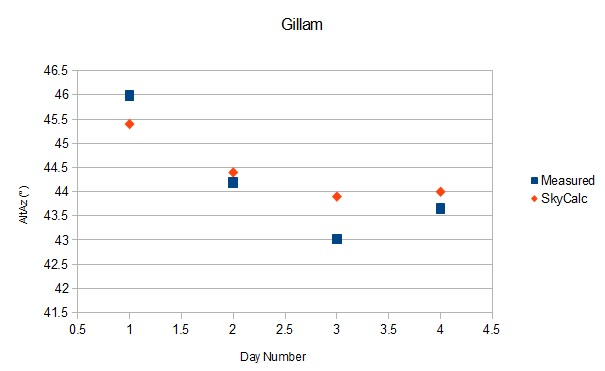
\includegraphics[scale=1.0]{gillam_AltAz_comparison.jpg}
\end{figure}

\begin{figure}[h!]
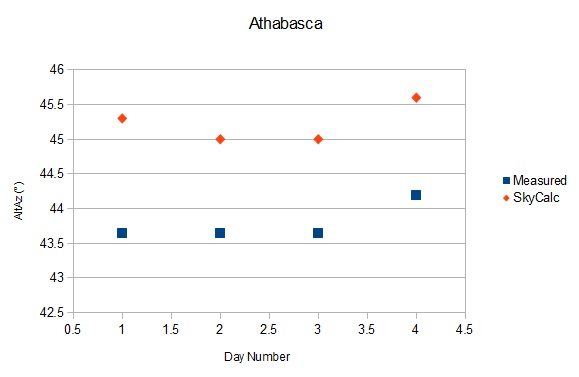
\includegraphics[scale=1.0]{athabasca_AltAz_comparison.jpg}
\end{figure}

\begin{figure}[h!]
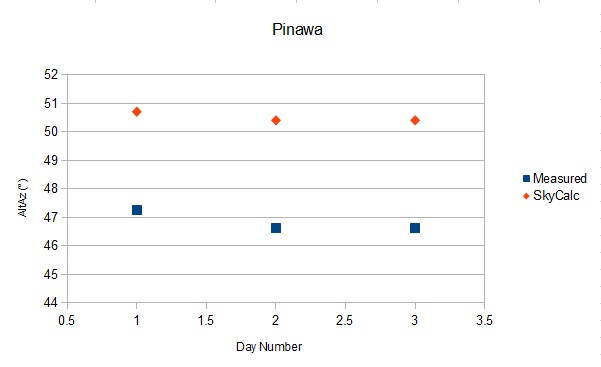
\includegraphics[scale=1.0]{pinawa_AltAz_comparison.jpg}
\end{figure}


\vspace{10mm}

\section{Results of AltAz Comparison}
\hspace{0.5cm}

All of the dates were chosen as far apart as possible. Unfortunately, most of the sights only have Jupiter visible at night from October to Febuary, which limits the window to work with considerably. Especially when data collection for a couple of the sites did not start until December. Nonetheless, the results were generally consistent with one another. The only exception was Gillam, which I personally have triple checked, and the plot is consistent with the data. The other sites are off the expected value from half a degree to about four degrees. Again, this is fairly reasonable as even with a perfect alignment there is an error of half a bin. Since each bin corresponds to about four degrees, an uncertainty of two degrees would be expected in a best case scenario. To obtain the real measured angles used in the plots, the "step\_variable17" file contains which bin number corresponds to a particular angle. There are 4000 steps per 360$^\circ$.

For the exact dates and other values used in producing the plots the spreadsheet is labeled "comparing Az at four sites." 

\section{Orientation Results}

Using the transit times also allowed me to analyze how far off the geographic north pole the camera was aligned. Plugging the transit time into SkyCalc gives an accurate result for the AltAz at a particular time and location. As discussed above, if the AltAz is 180$^\circ$ then the alignment is exactly on the geographic north pole. And as also discussed above, this turns out to not be the case. Below is a table comparing an average of the AltAz-180$^\circ$ with the current magnetic declination at each site. The results are at best somewhat consistent with the coordinates for each site, but unfortunately there are no concrete correlations . For all values of AltAz-180$^\circ$, they are averages from several nights data. All sites had extremely consistent data across the nights the data was averaged (\textless10\% differences between nights). The magnetic declination was found using the website "http://magnetic-declination.com/." All data used in producing the table is again in the spreadsheet "comparing Az at four sites."

\begin{center}
\begin{tabular}{| l | c | r| }
\hline
  Site & Az-180$^\circ$ & Mag. Declination \\ \hline
  Fort Smith & 10.1$^\circ$ & 16$^\circ$ 9' \\
  Athabasca & 15.15$^\circ$ & 15$^\circ$ 35' \\
  Gillam & 6.525$^\circ$ & 0$^\circ$ -23' \\
  Athabasca & 0.2667$^\circ$ & 2$^\circ$ 15' \\ \hline
\end{tabular}
\end{center}


\section{Conclusions}
\subsection{Consistency Across the Site's Imaging Process}
\hspace{0.5cm}

The three sites of Gillam, Athabasca, and Fort Smith appear to image Jupiter if not in exactly the same way across all filters, then close enough to be considered negligible for pretty much all data analysis performed using the instruments at the sites. The consistency between them is exactly what I was hoping to find. Pinawa, on the other hand, might be worth having someone look into what exactly is causing its discrepancy from the other sites. We did have a brief discussion and what the causes could be, and I believe the conclusion was that something was off with the lens system at the Pinawa site. This effect might not be relevant to the research being pursued, but it is definitely worth knowing.


\subsection{Orientation of the MSP's}

\hspace{0.5cm}

Looking at the Altazimuth of the sites and comparing it to the expected results using SkyCalc revealed most sites to be consistently off by a couple degrees. For Athabasca, Fort Smith, and Pinawa Jupiter is consistently lower by a degree or two across every night surveyed. My conclusion is that this a result of the leveling of the instruments being slightly off. As discussed, it is extremely hard to get an instrument exactly level in the field, and these results were about what I expected. However, there is no way to say what is causing the discrepenices with 100\% certainty unless someone goes out to the site to confirm or refute my conclusion. The important part is that the sites generally were off by a consistent amount, the exception being the site at Gillam. This is one area I would have liked to had more data and time to work with it. As easily seen in the Gillam plot, the difference in what was measured and what SkyCalc predicted are extremely inconsistent across the nights surveyed. This is something that is worth looking into, as I am not entirely sure what would be causing those particular results. Perhaps when the instrument that was malfunctioning at Gillam was replaced the orientation of the instrument changed. If this replacement occured between October 28th and November 20th 2011 than this is likely what happened. If the replacement occurred outside this time frame than I am not too sure what could explain the results. Like before, three sites are consistent with a fourth that might be worth looking into.

\indent For which direction the MSP's are pointed, I again found some irregularities. Having that that, the sites being pointed in different directions is completely expected. Jupiter's Az for every night surveyed at each site was always within a degree of one another, and usually within half a degree. The results of the Az-180$^\circ$ should be an accurate measure of the angular separation of the MSP's orientation off the geographic North-South meridian. This result should be especially useful if anyone needs to map an exact area of where something is occurring in the atmosphere.




\end{document}
\end{article}